\chapter{Baby MIND + WAGASCI}
\label{c:WAGASCI}

%Initially MIND prototype for nufact, now low pt can be used as muon spectrometry. Add preface to describe what done by xyz, clarify my contribution.
\section{Baby MIND}


%http://cds.cern.ch/record/2057587/files/SPSC-P-353.1.pdf

%Magnetized Iron Neutrino Detectors (MIND) have been operated in several experiments spanning 4 or so decades, such as CDHS, MINOS. These structures with magnetized steel plates interleaved with detector mod- ules are particularly well suited to provide large mass for neutrino experiments, and the characterization of the outgoing muon from νμ interactions, providing momentum measurements both by range and curvature, so in a sense self-calibrating, and providing charge identification. For this reason they have been naturally selected as baseline neutrino factory detectors.

%The Baby MIND project was launched as a prototyping activity within the European Commission-funded AIDA project with the principal aim to study muon charge identification efficiencies. The requirements that were set were correct sign background rejection to identify the wrong sign muon signature of a neutrino oscillation event at a Neutrino Factory.

 %In order to extend the neutrino factory capability to wrong- sign electrons, studies were made of totally active scintillator detectors (TASD) immersed in large volume magnetic field, in which sufficient tracking for electrons would allow charge separation. Since the scintillating detectors for the MIND and TASD are the same, the AIDA project foresaw to build a TASD prototype, immerse it in a large magnet available at CERN, and expose it to an electron beam.
 
%A MIND is planned for the recently approved WAGASCI experiment (T-59) at J-PARC on the T2K beamline to improve measurements of the ratio of neutrino interaction cross-sections on water and carbon motivated by the need to reduce systematics due to nuclear effects in water, currently the dominant systematic uncertainty in the T2K neutrino oscillation analyses. The size of the Baby MIND is particularly well suited for the WAGASCI experiment providing excellent acceptance for forward secondaries from interactions in the upstream WAGASCI water and carbon targets, Figure 1. The Baby MIND will be constructed and tested on a charged particle beamline at CERN. Once fully characterized, it will be shipped to J-PARC for operation with the WAGASCI experiment, where it is commonly referred to as the downstream Muon Range Detector (dMRD). Charge identification at much lower muon momenta in the T2K beamline is addressed by increasing the resolution on measurements of particle track angle rather than only providing position information.


%Magnetised Iron Neutrino Detectors (MINDs) have been proposed for Neutrino Factories, since wrong-sign muons are the neutrino oscillation signal. Baby MIND is a prototype detector to study charge identification of muons on a charged particle beamline at CERN. The CERN Neutrino Platform approved Baby MIND as experiment NP05 in December 2015 and construction started in August 2016 and finished in June 2017. 

The prototype Magnetized Iron Neutrino Detector (Baby MIND)~\cite{26babyMIND} was designed with the aim to study muon charge identification efficiencies in order to get estimates for a future Neutrino Factory, discussed in this section. The Baby MIND project was launched as a prototyping activity within the European Commission-funded AIDA project. The particle charge is essential for their oscillation measurements since wrong-sign muons are the neutrino oscillation signal. During the design process this a secondary aim was added, to measure the momentum and charge of muons from neutrino interactions in water and hydrocarbon targets at the J-PARC T59 (WAGASCI) experiment, further discussed in section~\ref{sec:WAGASCI}

The Baby MIND collaboration is comprised of 46 scientists from 10 different institutions, and is part of the CERN Neutrino Platform as experiment NP05~\cite{Fix2}.

\textbf{CHECK NUMBERS ABOVE!}

\subsection{Motivation}

The Baby MIND aims to show that MIND type detectors are viable to use for muon charge identification at low momenta ($<1$GeV/c) and also to show how well the charge can be identified from a Neutrino Factory~\cite{25NUfact} beam. Additionally the experiment aims to compare simulations from GEANT4~\cite{Geant4} to data taken from the detector to be able to verify the properties of muon interactions at momentum ranges of 0.5 to 10 GeV/c.

Separating and identify particles of different charges requires a magnetic field, and to perform identification at low momenta the a high uniform field has to be created for as large a volume as possible and preferably without fully stopping the particles which are being identified. The main difficulty comes from doing this in a cheap and simple way. \textbf{Mention Gas tpc!} In essence it creates a triangle where one can have a large magnetized volume over for instance gas, it will not stop particles but it will not be strong/cheap/large or uniform. The other option is to magnetize a large iron block which is cheap and uniform but stops particles.

For the Baby MIND a novel approach was chosen to use thin high quality magnetised ARMCO steel plates in an arrangement to optimize charge identification while minimizing the amount of steel plates surrounded by scintillator modules. The optimal design has been slightly shifted due to limiting constraints such as construction time, size of the ND280 shaft~\cite{21T2K} and design costs. An added advantage of this approach is the addition of a fully modular design leading to the Baby MIND being able to be set in any configuration with an appropriate support frame. By using magnetised steel modules instead of requiring the use of an all encompassing magnet, simplifies the magnetic design, lowers the cost and allows for a more uniform field. The direct disadvantages of this becomes the uncertainty of the momentum and difficulty of performing track reconstruction, discussed further in \textbf{Where?}.

The CERN Neutrino Platform approved Baby MIND as experiment NP05 in December 2015 and construction started in August 2016 and finished in June 2017. 

%During the development of the detector it was proposed to use Baby MIND as a muon spectrometer downstream of the WAGASCI experiment (T59) at J-PARC, using neutrinos from the T2K beamline, to provide charge and momentum of outgoing muons from neutrino charged current interactions. Currently the schedule is to install Baby MIND in the ND280 pit at the start of 2018.

 %the bending of the magnetic field to improve charge identification while using as few steel plates as possible.


%The Baby MIND spectrometer is designed to measure the momentum and charge of muons from neutrino interactions in water and hydrocarbon targets at the J-PARC T59 (WAGASCI) experiment. The WAGASCI experiment will measure the ratio of neutrino charged current interaction cross-sections on water and hydrocarbon aiming at reducing systematic errors in neutrino oscillation analyses at T2K. Construction of the Baby MIND detector within the CERN Neutrino Platform framework was completed in June 2017, where it underwent full commissioning and characterization on a charged particle beam line at the Proton Synchrotron experimental hall.

%The prototype is currently being built at CERN, where it will be provided with a charged particle test beam to fully understand the characteristics of the detector. Once the detector has been characterised, the plan is to integrate it into the WAGASCI experiment in Japan to improve measurements of the ratio of neutrino interaction cross-sections on water and carbon and also to place it downstream to provide improved charge identification. The main way of improving these measurements is by reducing systematic errors that arrive from the nuclear effects in water~\cite{26babyMIND}.

%History and use as low momentum spectrometer

\subsection{Layout}
\textbf{Project constraints for the design, construction and testing of the Baby MIND came from the need to operate the detector both at CERN and J-PARC on a relatively short timescale. Installation at J-PARC in particular has driven the overall design of the detector. The magnetisation scheme for the Baby MIND developed within the CERN Neutrino Platform framework is a direct result of the requirement to lower segments of detector elements through a narrow shaft down to the lowest floor of the ND280 building pit at J-PARC. } Image from nuphys poster!

Previous magnetised iron detector, discussed in chapter~\ref{c:expIntro}, have been in the kiloton range, Baby MIND is comparatively small weighing only 65 t. A schematic overview of the detector can be seen in \FigRef{fig:design}, showing the full detector composed of 18 scintillator modules, and 33 magnetised ARMCO steel plates, referred to as magnet modules. The full detector is around 4 meters in length with a height of around 2 meters and width of 3.5 meters. The current chosen layout of the detector is divided into four blocks with first block, block 1, containing 3 sub-blocks and the last block, block 4, containing 2 sub-blocks. The gaps between sub-blocks in block 1 have been added to improve the low momentum reconstruction using a lever-arm approach, discussed further in \textbf{Where?}.


%As discussed in \SubSectionRef{subsec:MINDdetector}, a MIND type detector requires a magnetized volume as well as interaction medium to deflect the particle tracks and scintillating elements to detect the particle hits. A schematic overview of the detector can be seen in \FigRef{fig:design}. 
\begin{figure}[h!]
\centering
%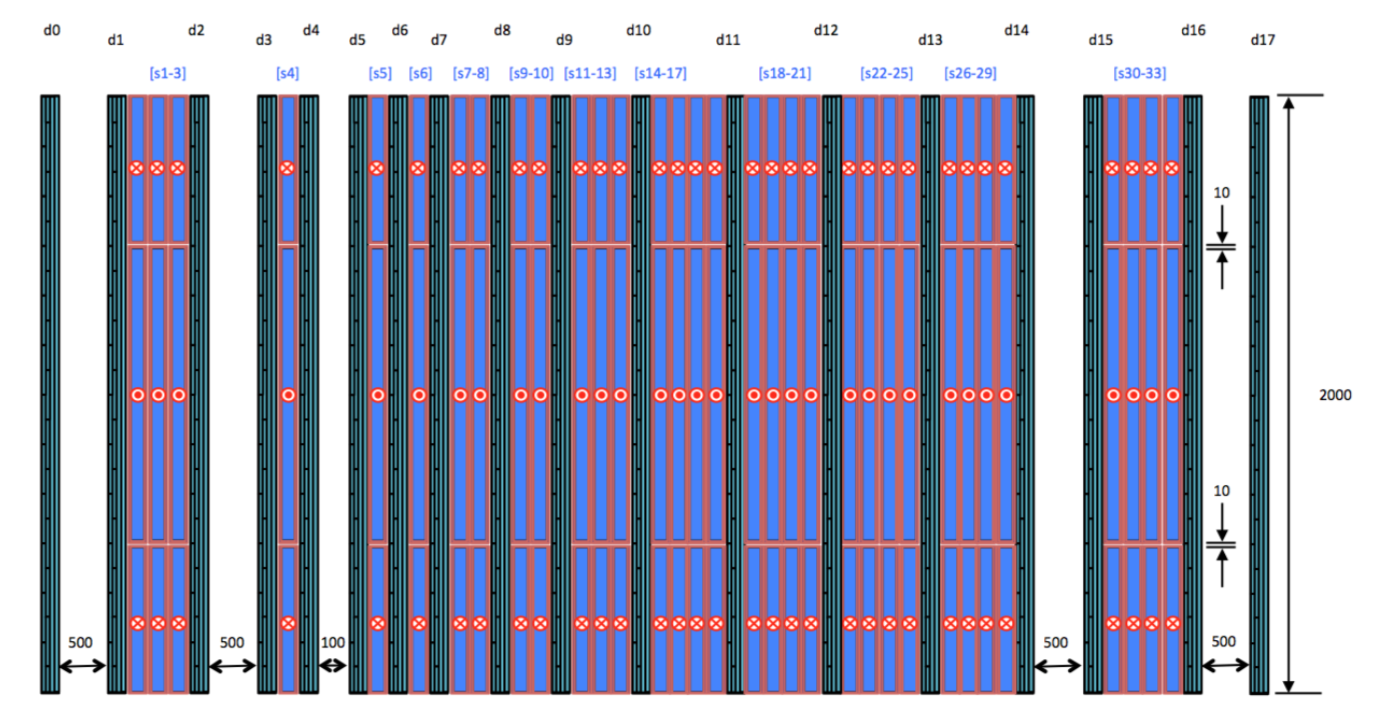
\includegraphics[width=\textwidth]{figures/design.png}
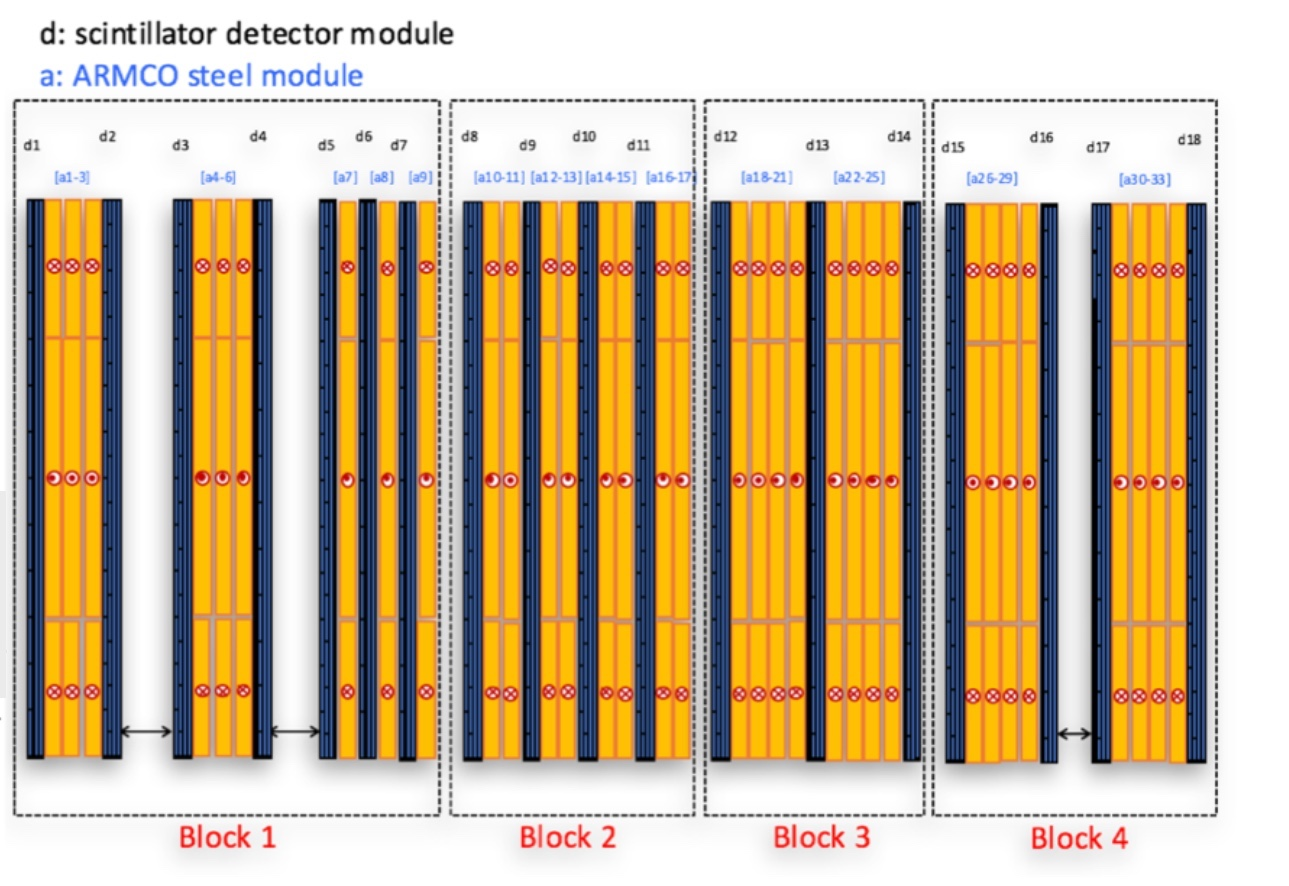
\includegraphics[width=\textwidth]{figures/MIND.jpeg}
\caption{The current Baby MIND design}
\label{fig:design}
\end{figure}

%Last layout
\textbf{iterations, highlight flexibility of design?}
\subsection{Magnet modules}

The magnetised volume for the Baby MIND has been chosen as a total of 33 steel modules both to have a simple magnetic field as well as being modular and cheaper than the alternatives. An overview of the magnetic field is seen in \FigRef{fig:mField} with two open slots in order to cover the entire plate with coils with currents in opposite directions. This improves the flux return, contains the stray fields and reduces power dissipation outside of the plates compared to a single conducting coil wound on the surface of each individual plate. Each module consists of ARMCO steel with two slits to allow aluminium coils to be wrapped around the steel and two side caps to allow for the magnetic flux return. The field is split into 3 parts where the field is 1.5 T but with opposite orientation as can be seen in \FigRef{fig:mField}. Because of this simple design, the field lines are contained in the steel and have negligible stray fields of less than 15 mT, with a good uniformity in the area of interest (seen as red in the \FigRef{fig:mField}). This provides a bending direction either up or down depending where the particle passes and its charge. The magnet module dimensions $3500 \times 2000 \times 30$ mm$^3$, with the field oriented in the x−direction (right) and bending with respect to the bend in z−axis (Into figure). Simulations show the magnet field map to be very uniform over this central tracking region covering an area of $2800 \times 2000$ mm$^2$, where the field component in the x−direction dominates with field in the other orthogonal directions. The magnet modules were constructed at CERN through the CERN Neutrino Platform~\cite{50MagnetMIND}.

Test results on the 33 modules show all to achieve the required field of 1.5 T for a current of 140 A, with a total power consumption of 11.5 kW.

%The Baby MIND is built from sheets of iron interleaved with scintillator detector modules. The 33 Baby MIND iron magnet modules are all individually magnetised, unlike traditional layouts for magnetised iron neutrino detectors (e.g. MINOS) which tend to be monolithic blocks with a unique pitch between consecutive iron segments and large conductor coils threaded around the whole magnet volume. This allows for far greater flexibility in the setting of the pitch between segments, and in the layouts that these detectors can take.

\begin{figure}[h!]
\centering
%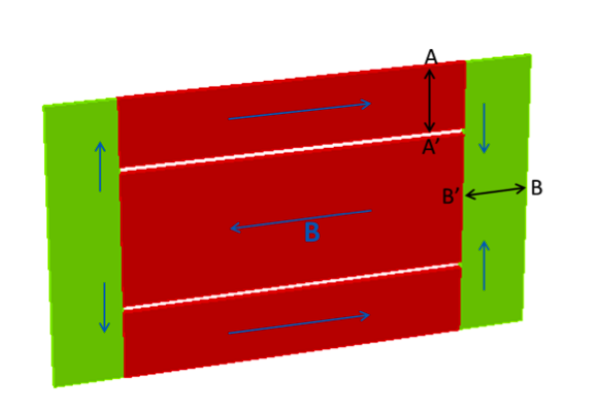
\includegraphics[width=0.45\textwidth]{figures/magnet.png}
%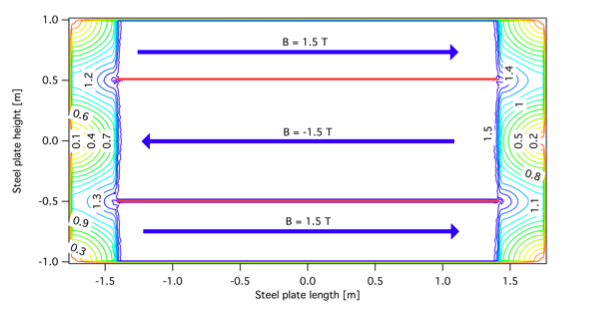
\includegraphics[width=0.45\textwidth]{figures/magnet2.png}
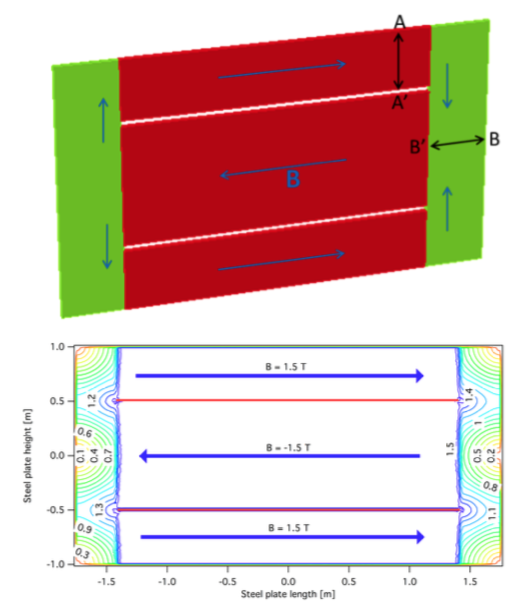
\includegraphics[width=\textwidth]{figures/Mfield.png}
%\caption{(Left) Schematic view of the magnet module. (Right) A contour plot of the magnet module, with the fiducial areas of interest showing magnetic field uniformity.}
\caption{(Top) Schematic view of the magnet module. (Bottom) A contour plot of the magnet module, with the fiducial areas of interest showing magnetic field uniformity.}
\label{fig:mField}
\end{figure}

\textbf{Field, credit in preface of CERN.}
\subsection{Scintillator modules}
In the Baby MIND, particle hits are detected by scintillating bars and provide both horizontal and vertical position information. There are a total of 18 scintillator modules, where each scintillator module is constructed from 95 horizontal bars, $3000 \times 31 \times 7.5$ mm$^3$, and 16 vertical bars, $1950 \times 210 \times 7.5$ mm$^3$ providing a total size of the scintillator module as $3000 \times 1950 \times 30$ mm$^3$. Since the vertical information is important for curvature, smaller bars are used to provide a better position resolution. The bars are arranged in 4 planes, of horizontal, vertical, vertical, horizontal, with an overlap between planes to achieve close to 100\% hit efficiency for minimum ionizing muons~\cite{51Saba}. INR Moscow built and designed the scintillator bars, providing a good light yield \textbf{figure ref!}, regardless of where the bar is hit. The bars are polystyrene based, 1.5\%PTP, 0.01\% POPOP and held together mechanically within an aluminium support frame  The bars contains Kuraray WLS fiber (200 ppm, S-type, diameter 1.0 mm) and contain a reflective coating 30 to 100 μm from chemical etching of surface. The connectors are custom made using Eljen EJ-500 optical cement. A schematic view of the horizontal bars can be seen in \FigRef{fig:horizontal} and the vertical bars in \FigRef{fig:vertical}. 


%The scintillating elements, seen in \FigRef{fig:Vbar}, have been chosen as 18 scintillating modules consisting of four planes per module, two oriented along the horizontal direction with and two oriented in the vertical direction, each to produce good horizontal and vertical resolution of the particle interactions 

\begin{figure}[h!]
\centering
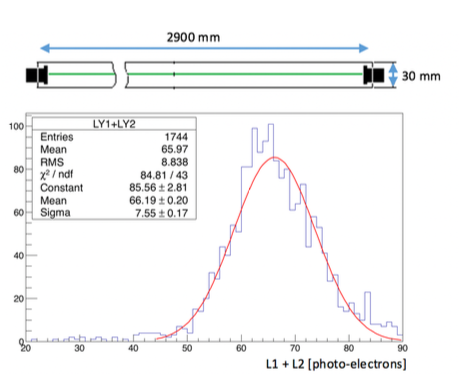
\includegraphics[width=\textwidth]{figures/horizontal.png}
\caption{Schematic view of the horizontal bar and light yield curves.}
\label{fig:horizontal}
\end{figure}


\begin{figure}[h!]
\centering
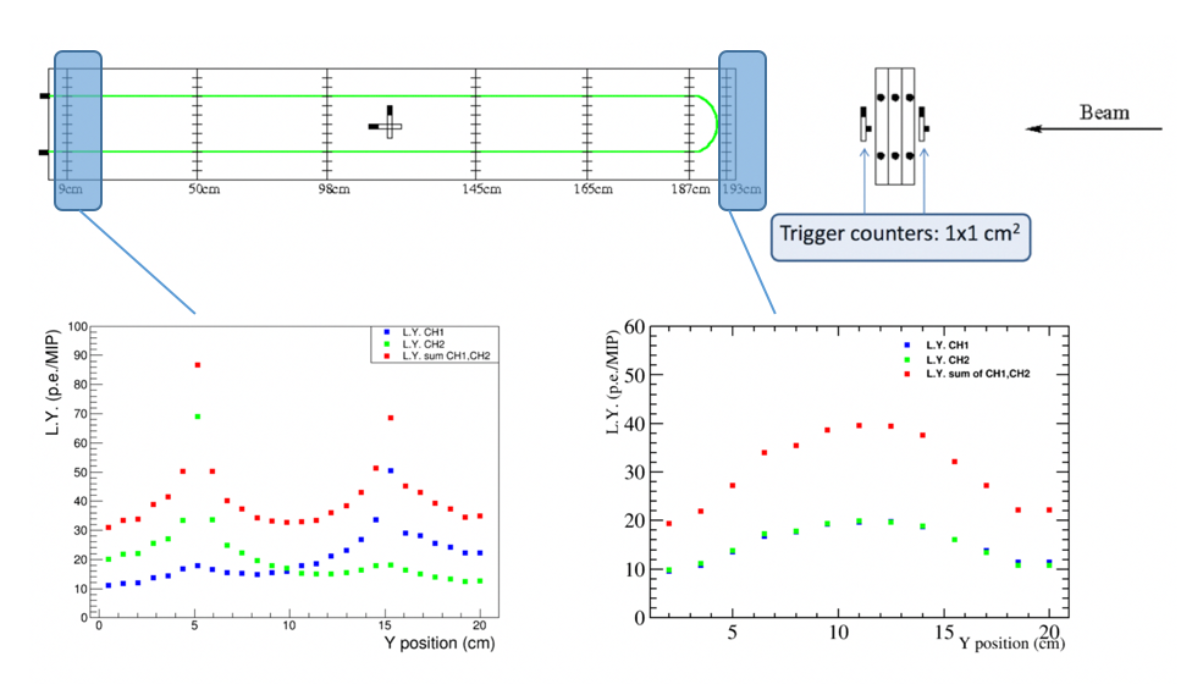
\includegraphics[width=\textwidth]{figures/vertical.png}
\caption{Schematic view of the vertical bar and light yield curves performed for hits at the near and far end of the bar.}
\label{fig:vertical}
\end{figure}


%\begin{figure}[h!]
%\centering
%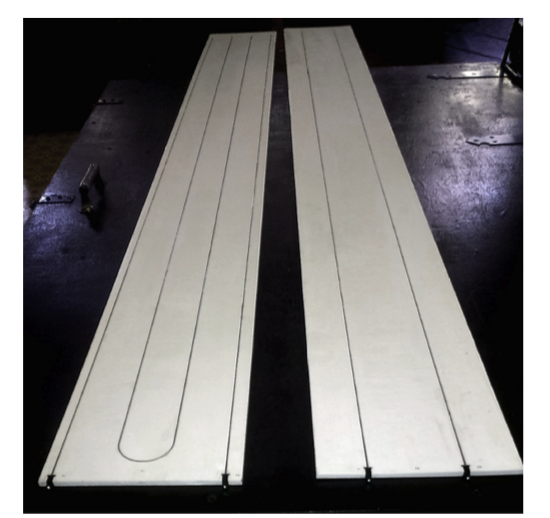
\includegraphics[width=0.5\textwidth]{figures/Vbar.png}
%\caption{One of the vertical scintillator bars.}
%\label{fig:Vbar}
%\end{figure}
\subsection{Electronics}
The scintillating fibres, present in the bars are read out using Hamamatsu MPPC (Multi Pixel Photon Counters). Compared to PMTs these use a lower voltage, less current and are compatible with magnetic fields. This provides a small size, and simple electronics for the modules. The MPPCs are custom made S12571-025C (and derived S10943-5796), a size of 1x1 mm2 (65\% fill factor) and 25 μm cell size. The operating voltage is ≈ 67.5 V with photon detection efficiency (PDE) ≈ 35\%, gain 5 × 105 and dark counts of typically 100 kcps. The MPPC signals, sampled at 400 MHz, are powered (HV/LV) and read out by custom made Front End Boards (FEBs), seen in \FigRef{fig:FEB}, designed for 96 channels using CITIROC ASICs. The MPPC signals are connected through a 5 m extension coaxial cable bundle containing up to 32 photosensors signals. The purpose is to decouple the FEBs from the scintillator modules, which improves accessibility to FEBs and their long term maintainability. These rack mounted FEBs have been designed by Geneva University containing $3 \times 32$ channel connectors, 3 CITIROC ASICs with 32 channels each. The FEBs are installed in mini-crates which can connect up to 7 FEBs via readout/slow control on USB3 and/or Gigabit using a backplane \FigRef{fig:crate}. 
Data is sent from the mini-crates to DAQ computers via USB3 and passed on to a final computer located in a control room. The full readout chain can be seen in the block diagram in \FigRef{fig:daqChain}.

%with a platform independent readout, Windows/Linux. There is also an analog readout, 8 μs for 96-channel low gain and high gain with a 12-bits, 8 channel, 40 MSam- ples/s per channel ADC based on the Altera ARIA5 FPGA. \textbf{Cite Etams paper?}

%with the readout electronics installed in 8 mini-crates on top of the detector. Each mini-crate can accommodate up to 7 Front-End Boards (FEB) (fig. 2). Each FEB can read-out up to 96 detector channels. The data is transferred to the Data Acquisition System (DAQ) via USB 3 interface. The FEBs can work either in standalone mode, in which every FEB is connected to the readout computer via a USB3 connection, or in time division multiplexing (TDM) mode in which all FEBs of a mini-crate are chained and the data is passed to a single USB3 master FEB which sends it to the DAQ. This allows sharing the available data bandwidth and reducing the amount of required cables. There also is a possibility, while in TDM mode, to assign the full USB bandwidth to any selected FEB in the chain.


\begin{figure}[h!]
	\centering
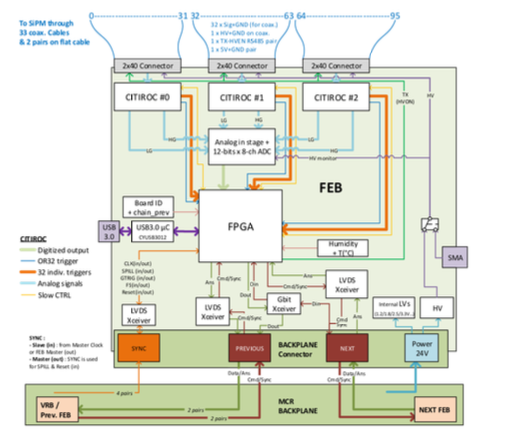
\includegraphics[width=0.48\textwidth]{figures/FEB.png}
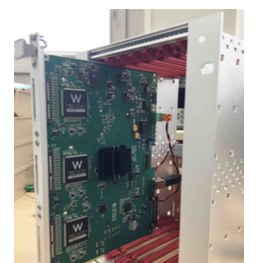
\includegraphics[width=0.48\textwidth]{figures/FEB2.png}
\caption{(Left) Schematic view of FEB layout. (Right) An image of the FEB in one of the racks.}
\label{fig:FEB}
\end{figure}

\begin{figure}[h!]
\centering
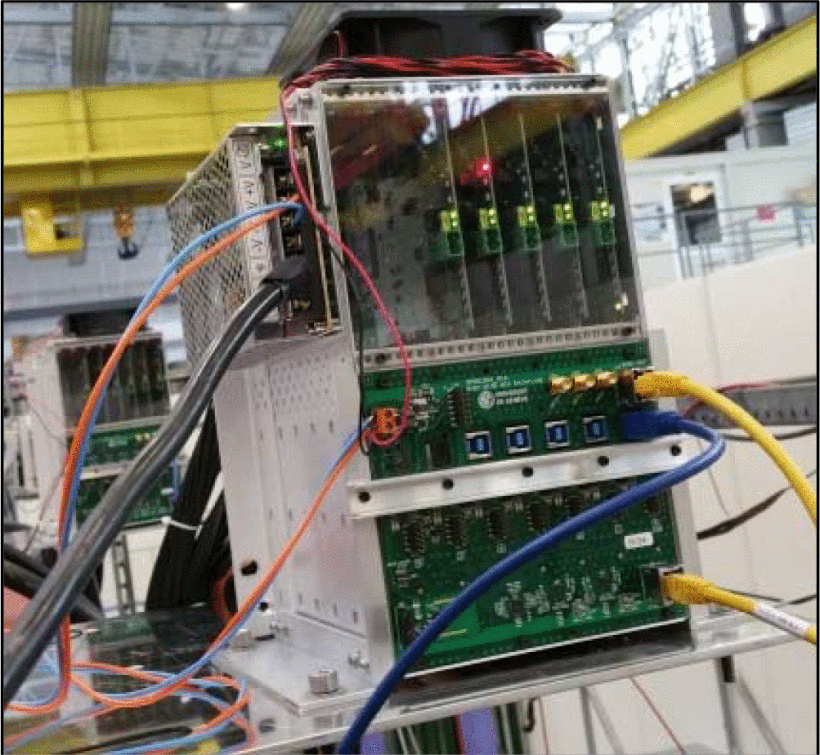
\includegraphics[width=0.48\textwidth]{figures/crateInstalled.png}
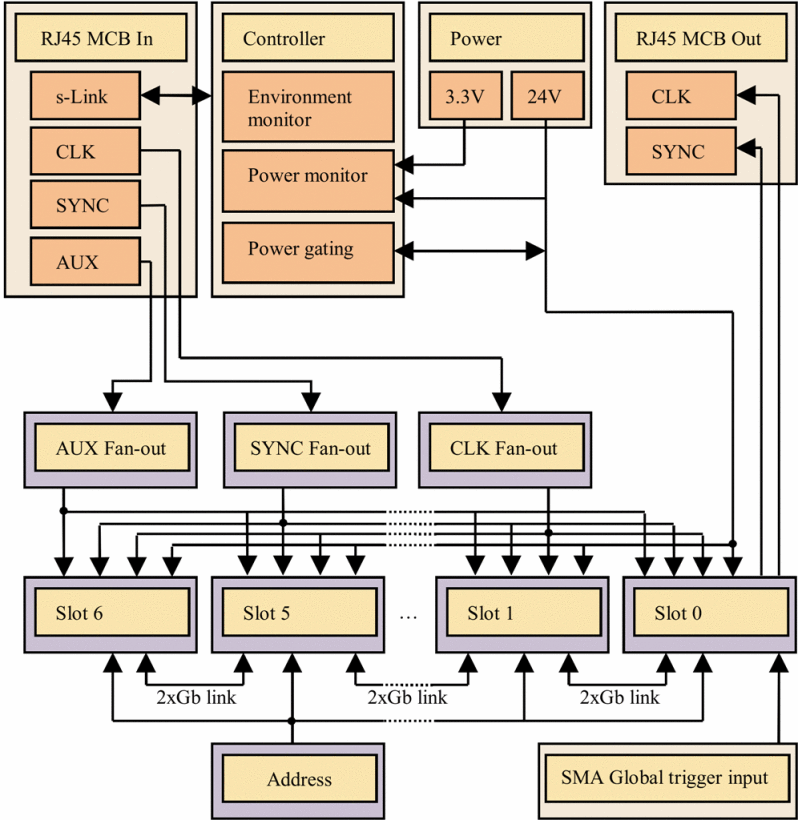
\includegraphics[width=0.48\textwidth]{figures/backplane.png}
\caption{(Left) Front end electronics mini-crate installed on the detector. (Right) Block diagram representing the backplane. Figures from \cite{52Georgi}}
\label{fig:crate}
\end{figure}

\begin{figure}[h!]
\centering
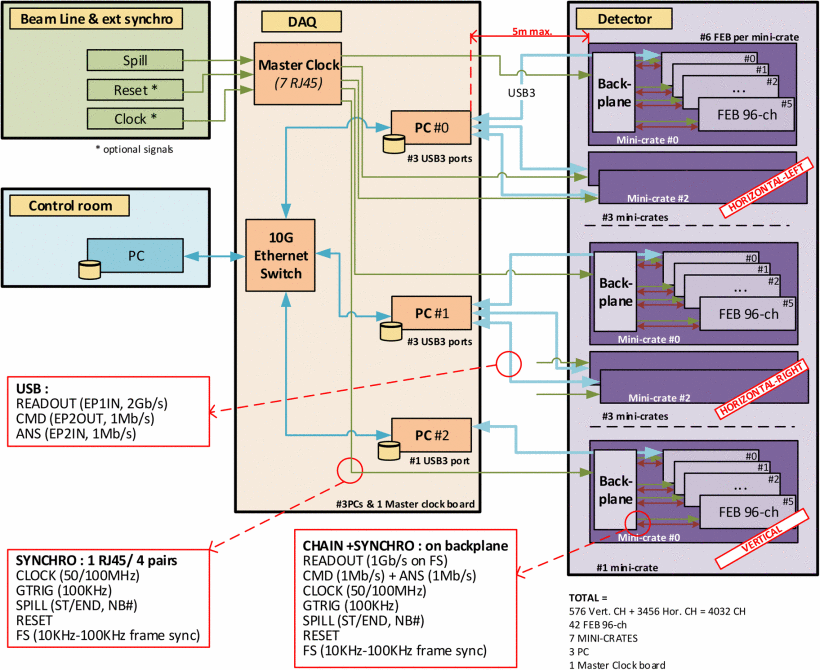
\includegraphics[width=\textwidth]{figures/fullDAQ.png}
\caption{Readout block for the Baby MIND. Figure from \cite{52Georgi}}
\label{fig:daqChain}
\end{figure}



%The Baby MIND electronic readout scheme includes several custom-designed boards [12].  At the heart of the system is the electronics Front End Board (FEB), developed by the University of Geneva, Figure 5. The readout system includes two ancillary boards, the Backplane, and the Master Clock Board (MCB) whose development has been managed by INRNE (Bulgarian Academy of Sciences) collaborators.
%One critical element in the photosensor readout path is the cable bundle, a 5 m extension coaxial cable RG174U that connects the photosensor to the FEB. Each bundle connects up to 32 photosensors. The purpose is to decouple the FEBs from the scintillator modules, which improves accessibility to FEBs and their long term maintainability. The module end of the bundle hosts some electronics that manages the application of the high voltage to the SiPMs, enabling faulty SiPMs to be switched off at that level. This feature was added after the summer 2016 beam tests, where a short circuit on a single channel would disable a bank of 96 channels.

%The FEBv2 hosts 3 CITIROC chips that can each read in signals from 32 SiPMs [13]. Each signal input is processed by a high gain, and a separate low gain, signal path. Both paths comprise independent pre-amplification and "slow" shaping stages with tuneable gain and shaping time con- stant, respectively. The outputs from the slow shapers can be sampled using one of two modes: a mode with an externally applied delay, and a peak detector mode. A faster shaper can be switched to either HG or LG paths, followed by discriminators with adjustable thresholds providing 32 individ- ual trigger outputs and one OR32 trigger output. An Altera ARIA5 FPGA on the FEBv2 samples these trigger outputs at 400 MHz, recording rising and falling times for the individual triggers and assigning time stamps to these. Time-over-threshold from the difference between falling and rising times gives some measure of signal amplitude, used in addition to charge information and useful if there is more than one hit per bar within the deadtime due to the readout of the multiplexed charge output of $\approx$ 9 μs. The ARIA5 also manages the digitization of the sampled CITIROC multiplexed HG and LG outputs via a 12-bit 8-ch ADC.

%The FEBv2 is designed to fit into a slot in a minicrate as shown in Figure 5. The front face receives the SiPMs cable bundles, the rear end plugs into the backplane. Up to 6 FEBv2 can be housed in each minicrate. Eight minicrates are distributed either side of the Baby MIND.
%The internal 400 MHz clock on the FEBv2 can be synchronised to a common 100 MHz clock. The synchronisation subsystem combines input signals from the beam line into a digital synchro- nisation signal (SYNC) and produces a common detector clock (CLK) which can eventually be synchronised to an external experiment clock [14]. Both SYNC and CLK signals are distributed to the FEBs. Tests show the FEB-to-FEB CLK(SYNC) delay difference to be 50 ps (70 ps). Signals from the beam line at WAGASCI include two separate timing signals, arriving 100 ms and 30 μs before the neutrino beam at the near detectors [15]. The spill number is available as a 16-bit signal.

\subsection{Construction and test beam}

The CERN Neutrino Platform approved Baby MIND as experiment NP05 in December 2015 and construction started in August 2016 and finished in June 2017. During the development of the detector it was proposed to use Baby MIND as a muon spectrometer downstream of the WAGASCI experiment (T59) at J-PARC, using neutrinos from the T2K beamline, to provide charge and momentum of outgoing muons from neutrino charged current interactions. \textbf{The installation and commissioning of the detector in J-PARC will took place in the beginning of 2018 and started to take beam at J-PARC in October 2018.}

\textbf{Discussion what was in the test beam, results in chap 5?}

\newpage

\section{WAGASCI}\label{sec:WAGASCI}

The new WAter- Grid-SCIintilator-detector (WAGASCI) being built at the J-PARC neutrino beam line will measure the difference in cross sections from neutrinos interacting with a water and scintillator targets, in order to constrain neutrino cross sections, essential for the T2K neutrino oscillation measurements. It follows a similar approach to the one used for Iron scintillator cross-sections in the INGRID detector~\cite{21T2K}.

Baby MIND will act as a magnetic spectrometer behind the main WAGASCI target. Baby MIND was installed inside the WAGASCI cavern at J-PARC in the beginning of 2018 to measure the charge and momentum of the outgoing muon from neutrino charged current interactions, to enable full neutrino event reconstruction in WAGASCI.

\subsection{Motivation}
The WAGASCI experiment (T-59) at J-PARC on the T2K beamline aims to improve measurements of the ratio of neutrino interaction cross-sections on water and carbon. This is required to reduce systematics due to nuclear effects in water, currently the dominant systematic uncertainty in the T2K neutrino oscillation analyses~\cite{21T2K} With planned upgrades to the T2K and planned follow-up project HyperK~\cite{24HyperK}, there is a strong motivation to reduce the systematic uncertainties. The aim is for T2K to improve the level of systematic precision to 4\%. 

%The main goals of the proposed detector are to improve the charge current cross section ratio between water and scintillator targets and to perform high-precision measurement of different charged current neutrino interaction channels.

WAGASCI proposes to test a new 3-D grid-type detector, composed of plastic scintillator and water, to improve on the current understanding of nuclear effects in neutrino interactions. The WAGASCI collaboration states that the detector will be able to measure this cross-section to a level of 3\% systematic uncertainties in the $1 GeV/c$ energy region with a generic MIND~\cite{30WAGASCI}, \textbf{however no evidence has been given for this claim}. Using WAGASCI as a near detector, in the ND280 building, combined with the far Cherenkov detector provides knowledge of the ratio of neutrino interaction cross-sections in water and plastic scintillator. Due to the design of the WAGASCI being both small and not including any magnets, it is impossible to reconstruct charge or momentum for incoming particles. By including the Baby MIND to provide reconstruction downstream, this obstacle is overcome. The size of the Baby MIND is particularly well suited for the WAGASCI experiment providing excellent acceptance for forward secondaries from interactions in the upstream WAGASCI water and carbon targets. During operation with the WAGASCI experiment, Baby MIND is referred to as the Muon Range Detector (MRD). The layout can be seen in \FigRef{fig:WAGASCI}.

%Long baseline neutrino oscillation experiments, amongst others, have confirmed the neutrino sector requires physics beyond the Standard Model. T2K (Tokai-to-Kamioka) discovered electron neutrino appearance in 2013 from a muon neutrino beam with a significance of 7.3σ with a frac- tion of the approved 7.8 × 1020 protons-on-target (POT) [1], using the Super-Kamiokande water Cherenkov located 295 km from the neutrino production site at the J-PARC. Results excluding zero CP violation at 90\% confidence level were announced by T2K in 2016, with data from 20\% of the approved POT. With upgrades to the proton beam, reaching 420 kW in 2016, and projected to reach 800 kW in 2019 and 1.3 MW beyond 2020, there is a strong motivation not to be systematics- limited for future runs at T2K and its follow-up project HyperK \cite{24HyperK}


%The T2K experiment requested an increase in exposure to 20 × 1020 POT, aiming to improve the level of systematic precision to 4\%. The J-PARC T59 experiment [3], referred to as "WAGASCI", will address one of the dominant uncertainties, the knowledge of the ratio of neutrino interaction cross-sections in water (far detector) and plastic scintillator (near detector).
%WAGASCI proposes to test a new 3-D grid-type detector, to improve on the current under- standing of multi-body nuclear effects of neutrino interactions in the 1 GeV energy region, possibly reaching a level of 3\% systematic uncertainties. 

%The 3-D modules have higher target fraction (80\%), and wider angular acceptance (4π) compared with the ND280 near detectors [4]. They are located on the B2 floor of the ND280 building, where different neutrino spectra are available from different off-axis positions. Measurements with different but fractionally overlapping beam spectra will help resolve contributions from different neutrino energies, important for oscillation analyses given the neutrino beam spectrum at a 2.5◦ off-axis angle is not monochromatic.

\begin{figure}[h!]
\centering
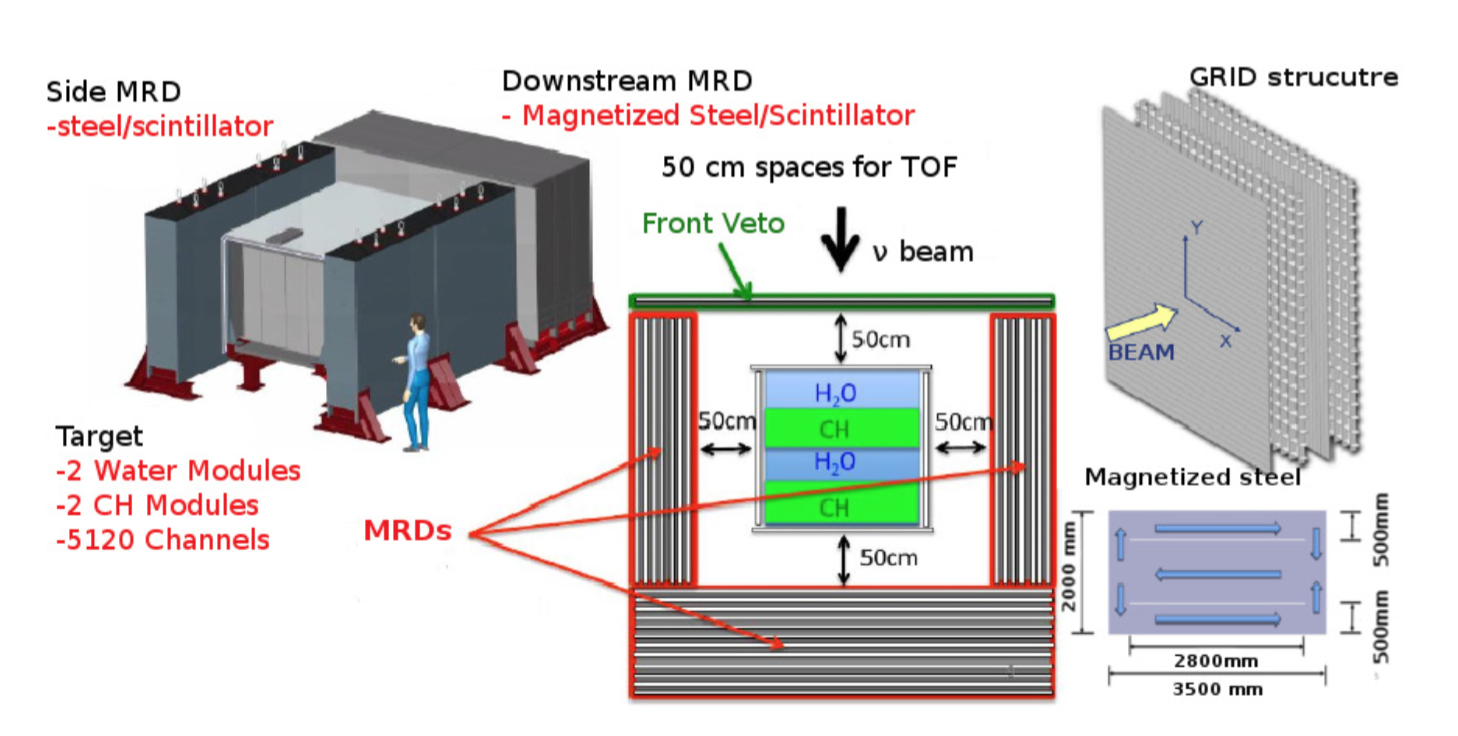
\includegraphics[width=\textwidth]{figures/WAGASCI.png}
\caption{The basic structure of the WAGASCI detector including one of the possible designs for the MIND plates. The MIND detector is denoted as Downstream MRD~\cite{30WAGASCI}.}
\label{fig:WAGASCI}
\end{figure}

\subsection{Layout}
There are two main elements of the WAGASCI, the central part is a neutrino interaction target which contains water and hydrocarbon, the target is surrounded by muon range detectors (MRDs). The main MRD, downstream of the target it the Baby MIND. The central part of WAGASCI, seen from above in the middle of \FigRef{fig:WAGASCI}, consists of four alternating modules filled with water or hydrocarbon. The main element is using a 3D-grid structure made of thin scintillator bars of $1000\times25\times3$ mm$^3$ each with boxes set in between. A side view can be seen in \FigRef{fig:StrucWAGASCI} and shows this clearer. The boxes are planned to be filled with water or scintillator and the size can be can be tuned to reach a compromise between the tracking granularity and the fraction of water over scintillator target. This design maximizes the fraction of the target material and also provides good particle tracking capabilities allowing to reconstruct tracks emerging at large angles w.r.t. neutrino beam direction.

\begin{figure}[h!]
\centering
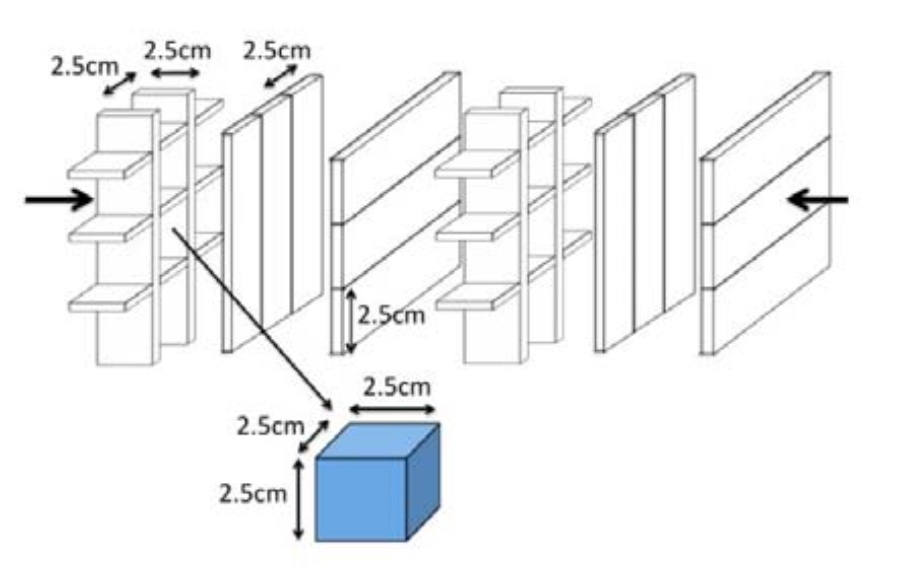
\includegraphics[width=\textwidth]{figures/structure.jpeg}
\caption{The structure of the WAGASCI detector with scintillator bars either horizontally or vertically with a structure to support each the boxes.}
\label{fig:StrucWAGASCI}
\end{figure}
%Plastic scintillator bars will be used as active elements in both target and surrounding muon range detectors. Light collection is done by utilizing WLS fibers (embedded into the grooves) that transport light to the photosensors, Hamamatsu MPPCs will be used for the latter. For WAGASCI experiment new generation of MPPCs will be used, these sensors have low dark noise rate, wider range of operation over-voltage (≃4V, allowing to increase the efficiency), and low rate of afterpulses and crorsstalk between the pixels.It is crucial to obtain high detection efficiency with thin bars of the target area so to fulfill the requirements of the physics program. The performance of plastic scintillator bars was measured with the 600 MeV positron beam. The average light yield was found to be 10-18 p.e. and the detection efficiency was better than 99\% for the whole region of scintillator with a threshold set to 1.5 p.e.The WAGASCI detector will collect data with both polarities of T2K focusing horn system. 

\subsection{WAGASCI target}
Already written about it above?
\subsection{MRD and Baby MIND}
The WAGASCI detector requires muon range detector to measure the momentum and charge of outgoing muons to identify the neutrino event and calculate the neutrino cross-section. As mentioned previously Baby MIND provides this role placed after the main target. There are also two much smaller MRDs on either side of the target to measure background muons from other sources or which have been produced from the neutrino beam but will miss the target or Baby MIND. These side MRDs will not be able to provide any momentum or charge information and will only be used as an extra veto plane for acceptance measurements. The layout can be seen in As seen in \FigRef{fig:WAGASCI}. The main event requirements are that the neutrinos decay somewhere in the target and produces a muon within a suitable angle to traverse four scintillator planes of the Baby MIND.

\subsection{Construction}
Unknown, is it built? No information given or public.

Preface, who did what?
\if{0}
\section{OLD}
\subsection{Timeline}
The current timeline for the construction of Baby MIND can be seen in \FigRef{fig:timeline}.
These are the following milestones expected to be met by the Baby MIND project:
\begin{itemize}
\item Beam tests characterization at CERN in May 2017.
\item Shipment to Japan in July 2017.
\item Installation in Japan,WAGASCI pit, in September for operation in October 2017.
\end{itemize}

\begin{figure}[h!]
\centering
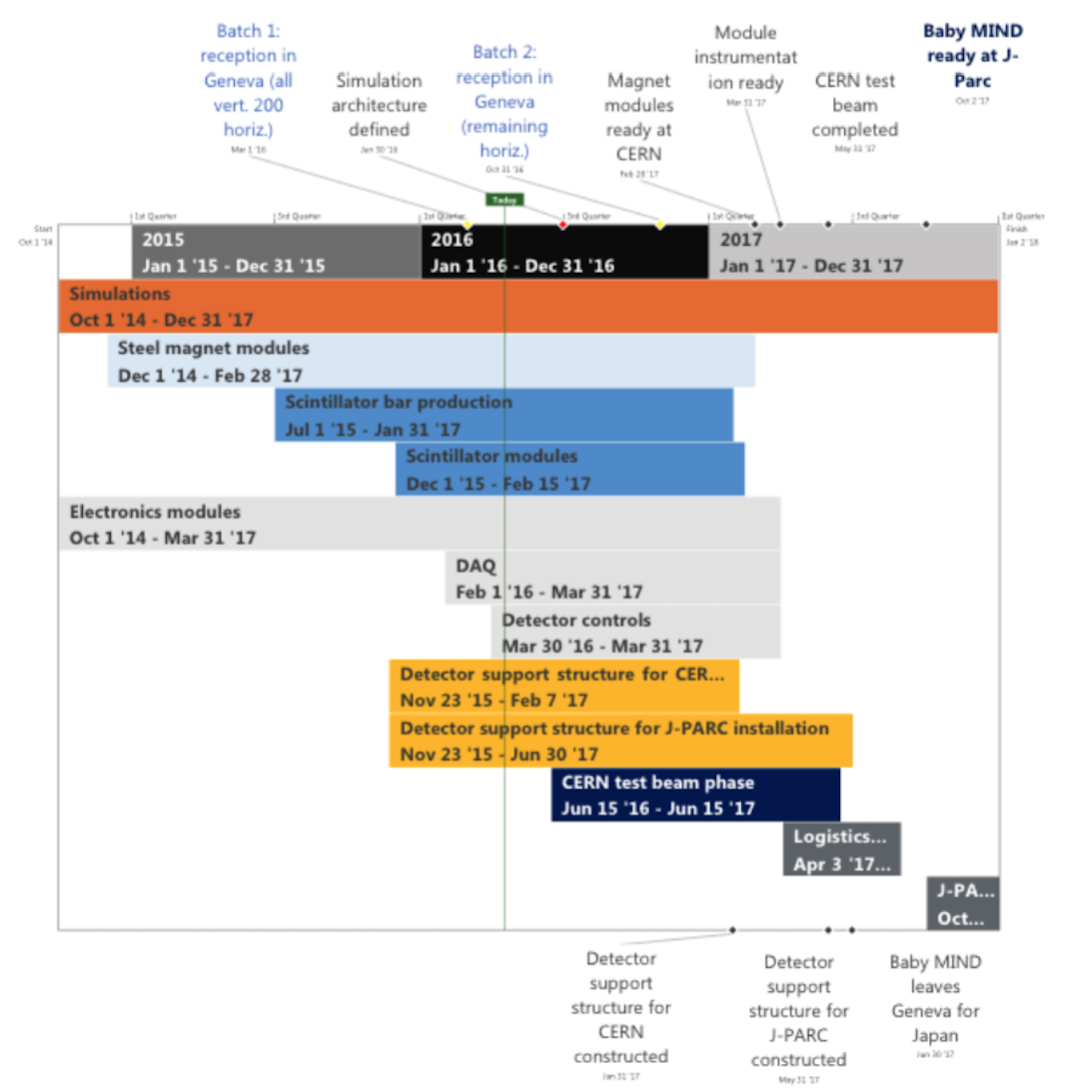
\includegraphics[width=\textwidth]{figures/timeline.png}
\caption{The current Baby MIND timeline}
\label{fig:timeline}
\end{figure}


\subsection{Collaboration}

\begin{figure}[h!]
\centering
\frame{
\includegraphics[width=\textwidth]{figures/Baby_MIND.png}}
\caption{The current Baby MIND collaboration}
\label{fig:collaboration}
\end{figure}

The 3000 Multi-Pixel Photon Counters (MPPC, also known as Silicon Photomultipliers, SiPM) were provided by the University of Glasgow. Glasgow is also responsible for the simulation software.
\subsection{Layout}

%\subsection{Motivation}
%In the white paper? LOI.

\section{WAGASCI/T59}



\subsection{Collaboration}

The current WAGASCI collaboration is given in figure~\ref{fig:collaborationW}.
\begin{figure}[h!]
\centering
\frame{
\includegraphics[width=\textwidth]{figures/T59_collaboration_18April2017.pdf}}
\caption{The current WAGASCI collaboration}
\label{fig:collaborationW}
\end{figure}

\subsection{Layout}
A new water-scintillator detector, WAGASCI (WAter- Grid-SCIintilator-Detector) seen in figure~\ref{fig:WAGASCI}, is proposed to reduce the systematic error in the T2K neutrino experiment.

\begin{figure}[h!]
\centering
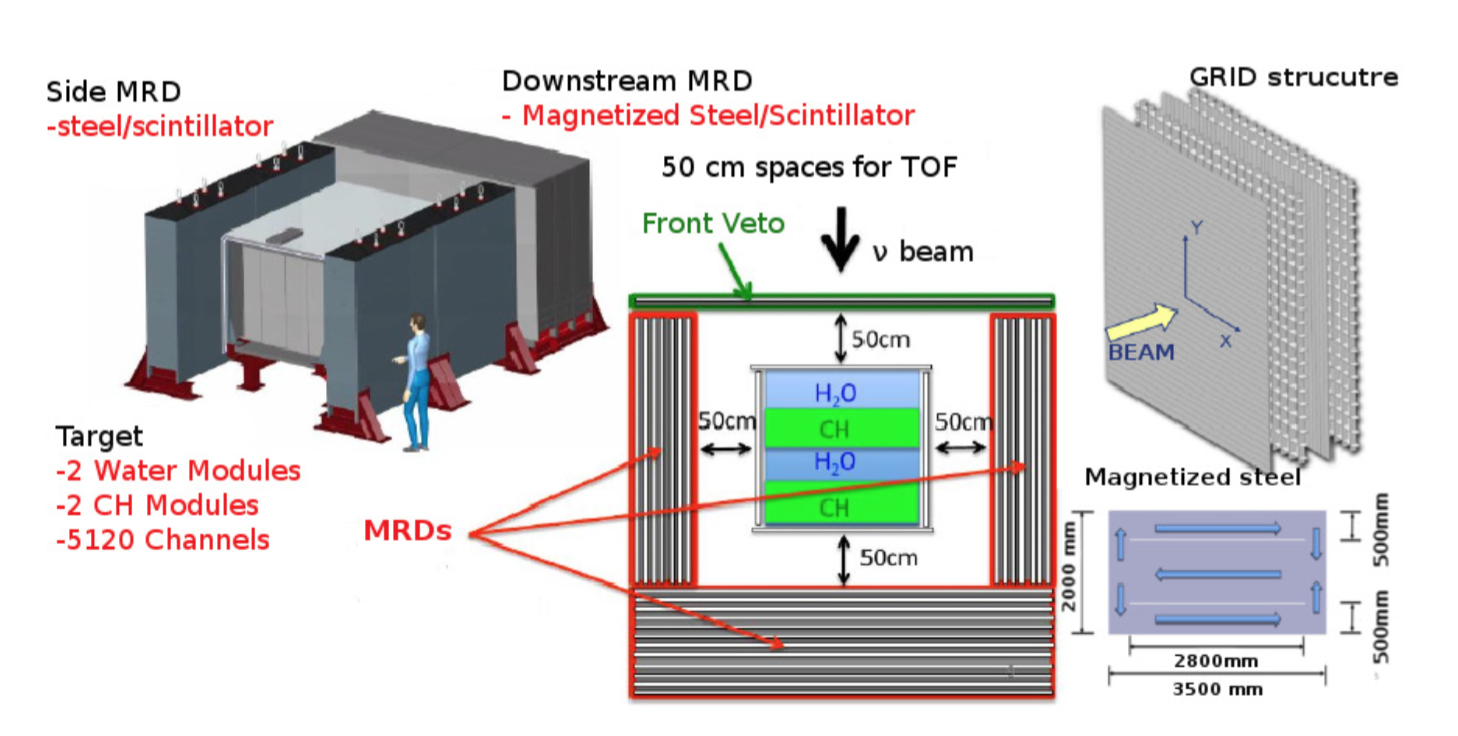
\includegraphics[width=\textwidth]{figures/WAGASCI.png}
\caption{The basic structure of the WAGASCI detector including one of the possible designs for the MIND plates.~\cite{30WAGASCI}.}
\label{fig:WAGASCI}
\end{figure}

\subsection{Motivation}
The main goals of the proposed detector are to improve the charge current cross section ratio between water and scintillator targets and to perform high-precision measurement of different charged current neutrino interaction channels.

\fi
